%% TeXworks instructions:
% !TeX root = ./report.tex
% !TEX encoding = UTF-8 Unicode
%% !TEX program = arara
%% !TEX TS-program = arara
% !TeX spellcheck = it-IT

% arara: pdflatex: { synctex: yes, action: batchmode, options: "-halt-on-error -file-line-error-style" }
% arara: pdflatex: { synctex: yes, action: nonstopmode, options: "-halt-on-error -file-line-error-style" }

%% Generate a report.xmpdata file with title and authors for PDF/A-compliant format %%
\begin{filecontents*}{\jobname.xmpdata}
    \Title{Maraph1-mp Project Report}
    \Author{Nicholas Brasini\sep Gjulio Jakova\sep Federico Naldini\sep Jacopo Riciputi}
\end{filecontents*}

\documentclass[%
    a4paper,            % specifica il formato A4 (default: letter)
    10pt,               % specifica la dimensione del carattere a 10
    oneside,            % serve per impaginare per stampa solo fronte
    notitlepage         % mette il titolo in una pagina separata (solo per article)
]{article}

\usepackage{a4wide}             % consente di avere più spazio nell'A4

%% ORDINE IMPORTANTE INIZIO %%%%%%%%%%%%
\usepackage[T1]{fontenc}        % serve per impostare la codifica di output del font
\usepackage{textcomp}           % serve per fornire supporto ai Text Companion fonts
\usepackage[utf8]{inputenc}     % serve per impostare la codifica di input del font
\usepackage[
    english,            % utilizza l'inglese come lingua secondaria
    italian             % utilizza l'italiano come lingua primaria
]{babel}                        % serve per scrivere Indice, Capitolo, etc in Italiano

\usepackage{lmodern}            % carica una variante Latin Modern prodotto dal GUST
%% ORDINE IMPORTANTE FINE %%%%%%%%%%%%%%

\usepackage{indentfirst}        % serve per avere l'indentazione nel primo paragrafo
\usepackage{setspace}           % serve a fornire comandi di interlinea standard
\usepackage{xcolor}             % serve per la gestione dei colori nel testo
\usepackage{graphicx}           % serve per includere immagini e grafici

\graphicspath{{./images/}}

\usepackage[%
    strict,             % rende tutti gli warning degli errori
    autostyle,          % imposta lo stile in base al linguaggio specificato in babel
    english=american,   % imposta lo stile per l'inglese
    italian=guillemets  % imposta lo stile per l'italiano
]{csquotes}                     % serve a impostare lo stile delle virgolette

\usepackage{multirow}           % aggiunge la possibilità di raggruppare celle su più righe nelle tabelle

\onehalfspacing%                % Imposta interlinea a 1,5 ed equivale a \linespread{1,5}

\setcounter{secnumdepth}{4}     % Numera fino alla sottosezione nel corpo del testo
\setcounter{tocdepth}{4}        % Numera fino alla sotto-sottosezione nell'indice

\usepackage[%
    depth=3,            % equivale a bookmarksdepth di hyperref
    open=false,         % equivale a bookmarksopen di hyperref
    numbered=true       % equivale a bookmarksnumbered di hyperref
]{bookmark}                     % Gestisce i segnalibri meglio di hyperref
\usepackage{hyperref}           % Gestisce tutte le cose ipertestuali del pdf
\hypersetup{%
    pdfpagemode={UseNone},
    hidelinks,          % nasconde i collegamenti (non vengono quadrettati)
    hypertexnames=false,
    linktoc=all,        % inserisce i link nell'indice
    unicode=true,       % only Latin characters in Acrobat’s bookmarks
    pdftoolbar=false,   % show Acrobat’s toolbar?
    pdfmenubar=false,   % show Acrobat’s menu?
    plainpages=false,
    breaklinks,
    pdfstartview={Fit},
    pdfauthor={Nicholas Brasini, Gjulio Jakova, Federico Naldini, Jacopo Riciputi},
    pdfcreator={Nicholas Brasini, Gjulio Jakova, Federico Naldini, Jacopo Riciputi},
    pdftitle={Maraph1-mp Project Report},
    pdflang={it}
}
\usepackage[utf8]{inputenc} % serve per avere l'indice di tutti i capitoli all'inizio 

%\usepackage[a-1b]{pdfx}
\usepackage[%
    english,italian,    % definizione delle lingue da usare
    nameinlink          % inserisce i link nei riferimenti
]{cleveref}                     % permette di usare riferimenti migliori dei \ref e dei varioref

\title{\LARGE{\textbf{Maraph1-mp Project Report}}}

\author{%
    Nicholas~Brasini\\%
    Gjulio~Jakova\\%
    Federico~Naldini\\%
    Jacopo~Riciputi
}

\date{%
    \small{Paradigmi di Programmazione e Sviluppo}\\%
    \small{Anni accademici 2017--2018 e 2018--2019}
}


\begin{document}
	
    \maketitle
    \clearpage
	\tableofcontents
	\clearpage
    \section*{\Huge {Capitolo 1}\label{chapter1}}
      \section{Processo di sviluppo}\label{sec:process}
        \subsection {Metodologia di sviluppo}\label{subsec:metodology}
        \subsection {Strumenti adottati}\label{subsec:tools}
        
        \clearpage
        
    \section*{\Huge {\textbf Capitolo 2}\label{chapter2}}
    \section{Requisiti}\label{sec:requirements}
         \subsection {Requisiti utente}\label{subsec:requirements:business}
             \subsection {Requisiti funzionali}\label{subsec:requirements:functional}
            \subsubsection[Gioco]{\large {Regole del gioco}\label{subsub:requirements:game}}
            \subsubsection[NoAutenticazion]{\large {Servizio di gioco senza autenticazione}\label{subsub:requirements:noauth}}
            \subsubsection[Autenticazion]{\large {Servizio di gioco con autenticazione}\label{subsub:requirements:auth}}
            \subsubsection[Stanze di gioco]{\large {Servizio delle stanze di gioco}\label{subsub:requirements:lobby}}
            \subsubsection[Interfaccia utente]{\large {Interfaccia grafica per l'utente}\label{subsub:requirements:gui}}
        \subsection {Requisiti non funzionali}\label{subsec:requirements:notFunctional}
        \subsection {Requisiti implementativi}\label{subsec:requirements:implementative}
   
   \clearpage
    \section*{\Huge {\textbf Capitolo 3}\label{chapter3}}
    \section{Design architetturale}\label{sec:design}
       
        
        \subsection[Architettura]{Architettura e pattern utilizzati}\label{subsec:architecture}
         L'architettura del sistema si basa fortemente su un design client-server. 
        Mentre per la realizzazione dell'applicazione locale è stato adottato il pattern Model-View-Controller, così da permettere una maggior suddivisione dei compiti, soprattuto per quanto riguarda la parte grafica e logica del gioco dalla sezione di interazione con il remoto. 
        Per il lato server-side invece, dato che le specifiche, oltre che a richiedere una parte statica, di semplice gestione dati, richiedevano anche una parte dinamica (real-time), sono stati adottati due differenti pattern. 
        \\
        La gestione dei dati è stata affidata ad un server che mette a disposizione per i client una serie di chiamate \textbf{API REST}, mentre per il real-time la scelta è ricaduta sulla creazione di una sessione di gioco utilizzando il pattern \textbf{Publish-Subscribe}.
        
        
            \subsubsection{Architettura server-side}\label{subsub:architecture:server}
            Nonostante l'architettura del server non sia a microservizi, si è preso spunto dalle loro potenzialità per costruire un modello che sia in futuro facilmente scalabile. 
            \\
            Per fare ciò è stato inserito tra il client e il backend un \textbf{Service discovery}. 
            
            \begin{figure}[h!]
                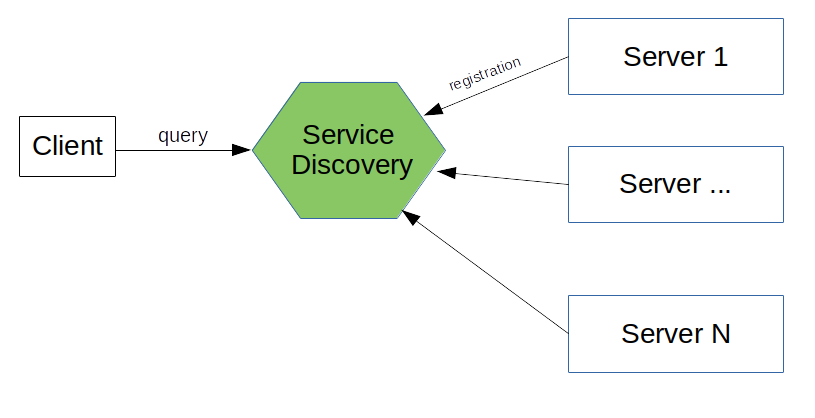
\includegraphics[width=\linewidth]{image/ArchitetturaDiscovery.png}
                \caption{Architettura client-server con Service Discovery. Allo start up il server si iscriver sul discovery e si rende disponibile, a questo punto il discovery lo considererà come componente attivo e vi indirizzerà i client.}
            \end{figure}

            Grazie al Discovery è stata data, a livello di modello, la possibilità all'applicazione di aggiungere servizi e di avere anche più server che si occupano dello stesso dato che, essendo il discovery l'intermediario tra il client e il server funge anche da Load Balancer, andando perciò a indirizzare il client verso il servizio con meno carico al momento della chiamata.
            In questo modo l'applicazione risulta essere altamente scalibile oltre che fornire high availability e una buona tolleranza al fallimento. 
            \\
            Una volta ottenuto un instradamento verso uno dei server disponibili entra in gioco un classico servizio ad API REST che si occupa della gestione dell'utente, sia per la parte social che per la ricerca di una partita. 
            
            A questo punto l'architettura utilizzata cambia. Le richieste del dominio impongono una sessione di gioco attiva capace di mantenere uno stato e le API REST non risultano la miglior soluzione. 
            Per la costruzione di un dialogo in real-time fra tutti i componenti di una partita e il server, che gioca nel ruolo di manager di quest'ultima è stato adottato, come anticipato, il pattern Publish-Subscribe. 
            In questo modo ogni membro della partita in ascolto su di un determinato canale sono capaci di ricevere ed emettere messaggi cosicchè, alla produzione di un dato da parte di uno dei partecipanti, tutti gli altri siano capaci di recepirlo e consumarlo per poi eventualmente rispondere tramite una determinata azione.
            
            \begin{figure}[h!]
                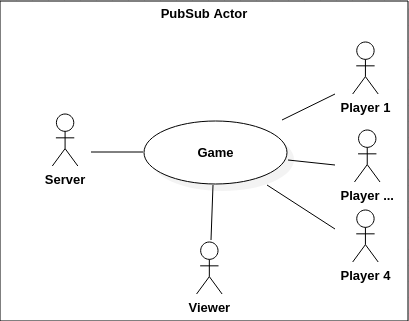
\includegraphics[scale=0.6]{image/PubSubActorDiagram.png}
                \caption{Attori attivi all'interno di un topic del Publish-Subscribe. Il questo caso il topic è inerente ad una partita.}
            \end{figure}
            
            \subsubsection{Architettura client-side}\label{subsub:architecture:client}
            Lato client come indicato è stato addottato il pattern MVC. Data la struttura del progretto questa architettura ha permesso uno sviluppo ben distinto delle parti.
            \\
            L'utente infatti, come è possibile vedere dalla figura \ref{fig:UserUseCaseDiagram}, viene indirizzato verso pià funzionalità:
            \begin{itemize}
             \item Interfaccia di login o registrazione;
             \item Interfaccia social;
             \item Schermata di gioco.
            \end{itemize}
            Sfruttando i vantaggi del il pattern \textbf{Model-View-Controller} sono stati anche identificati degli attori per la gestione delle parti, così da avere un dialogo tra parte grafica e controller reattiva. 
            La parte di modello invece offre le funzionalità necessarie per gestire al meglio le chiamate al backend per la parte social oltre che per la gestione delle partite vere e proprie.
            
            
	     \begin{figure}[!h]
                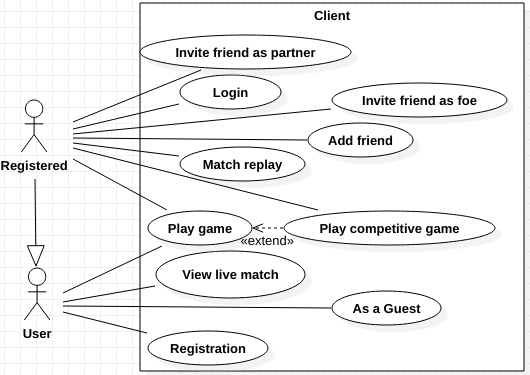
\includegraphics[scale=0.7]{image/UserUseCaseDiagram.png}
                \label{fig:UserUseCaseDiagram}
                \caption{Diagramma dei casi d'uso per le due differenti tipologie d'utente.}
            \end{figure}
            
            


        \subsection{Tecnologie}\label{subsec:technologies}
        Diseguito l'elenco delle tecnologie più rilevanti utilizzate per l'implementazione del progetto.
	  \subsubsection{JavaFX}\label{subsub:tecnologie:javafx}
	    Libreria grafica tra le più importanti nel mondo Java, se non la più importante. 
	    \\
	    La scelta è ricaduta su di essa in quanto ritenuta più facilmente integrabile con l'idea implementativa. 
	    La dinamicità con il quale è possibile definire file FMXL e la netta suddivisione tra view e controller l'hanno resa per il nostro progetto un'ottima alternativa a Swing.
	    La sezione di JavaFX rappresenta anche l'unica parte scritta in Java, in quanto il framework è stato considerato più maturo rispetto alle librerie disponibili in Scala.
	    
	 \subsubsection{Akka}\label{subsub:tecnologie:akka}
	   Sia lato client che lato server è stato utilizzato il framework Akka per la gestione degli attori. 
	   Le capacità di questa libreria di astrarre aspetti complicati di computazione hanno permesso lo sviluppo di un applicazione reattiva su entrambe le parti con il minimo sforzo. 
	   
	 
	 \subsubsection{Akka Cluster}\label{subsub:tecnologie:akkacluster}
	   La realizzazione di un dialogo dinamico tra i client e il server ci ha guidati verso il pattern \textbf{Publish-Subscribe}, per questo motivo la nostra scelta è ricaduta su Akka Cluster. 
	   \\
	   Essendo ben definita un'architettura client-server si è optato per seguire la strada inglobarla all'interno di un cluster cosicchè lo scambio di messaggi, tra il client e il server, non avvenga in modalità peer-to-peer.
	   \textbf{Akka Cluster} va inoltre ad aggiungere un'ulteriore scalabilità e affidabilità del sistema dato che, per sua natura, gestisce l'entrata dei nodi nel cluster e i loro ruoli, oltre che a monitorarne le prestazioni e l'eventuale caduta di essi. 
	 \subsubsection{Vert.x}\label{subsub:tecnologie:vert.x}
	  Libreria utilizzata per la gestione del server remoto. Il servizio REST è interamente costruito su Vert.x e lato cliente le stesse chiamate alle API si appoggiano alla parte client della libreria.
	  Tra gli altri si è optato per Vert.x, oltre che per la sua struttura che si basa sugli eventi asincroni all'interno di un event-loop, per la sua semplicità di deploy. A differenza di altri web server più conosciuti all'interno del mondo Java o Scala come Java EE o Spring, Vert.x è totalmente
	  indipendente e non necessita di un servlet container, permettendo perciò un deploy più immediato.
        \clearpage
        
	 \subsubsection{Cornhicon} 
	  TODO
    \section{Design di dettaglio}\label{sec:design:details}
    
    \clearpage
    
    \section{Implementazione}\label{sec:implementation}
        \subsection{Nicholas Brasini}\label{subsec:brasini}
        \subsection{Gjulio Jakova}\label{subsec:jakova}
        \subsection{Federico Naldini}\label{subsec:naldini}
        \subsection{Jacopo Riciputi}\label{subsec:riciputi}
	  Lo studente Jacopo Riciputi si è dedicato per la maggior parte del progetto nello sviluppo del servizio di server remoto e gestione dei dati e, in minor parte, di una prima implementazione delle regole di gioco. 
	  \\
	  Nel dettaglio: 
	    \begin{itemize}
	     \item Configurazione di TravisCI;
	     \item Generazione dei Jar;
	     \item Definizione delle regole di gioco;
	     \item Backend;
	     \item Client per richieste HTTP;
	     \item Ricerca di una partita;
	     \item Gestione dei dati
	    \end{itemize}
	    
	
	\subsubsection{Configurazione di TravisCI}
	  La configurazione di Travis è risulta fin da subito molto semplice, in quanto il servizio è stato utilizzato con l'unico scopo di effettuare i test ad ogni push sul repository.
	 
	\subsubsection{Generazione dei Jar} 
	  Per la generazione dei Jar ci si è affidati al plugin \textbf{shadow} che tramite il task sahdow jar
	  offre la possibilità di generare \textit{fatJar} completi e pronti all'esecuzione semplicemente definendo preventivamente qualche variabile. \\
	  È nata qualche difficoltà nel momento in cui si aveva la necessità di generare tre jar differenti, uno per ogni main presente nel progetto. 
	  Per fare ciò sono stati definiti all'interno del file \textit{build.gradle} tre task, uno per main, all'interno dei quali viene gestito \textbf{ShadowJar} 
	  al quale per task viene definito un classificatore da associare al jar da creare, la \textit{main class} 
	  e vengono ereditate le dipendenze dal \textit{shadow jar} principale.
	  
	\subsubsection{Definizione delle regole di gioco}
	  Lo scopo iniziale del primo sprint era quello di ottenere una modalità base di gioco nel quale fossere definite le basiche funzionalità aspettate, senza prendere in considerazione l'aspetto distribuito.
	  \\
	  Durante questa sezione mi sono occupato delle sviluppo di una prima versione di quello che poi successivamente è diventato il GameActor, gestore dell'intera partita. 
	  Per fare ciò sono partito subito dalla definizione di un semplice trait che però definisse gli aspetti principali il gioco doveva rispettare. 
	  Il trait in questione è \textbf{Match}. Una volta definito questo trait, nonostante la sua semplicità, il suo sviluppo a portato di conseguenza alla definizione di tutti gli aspetti di gioco ad esso legati. 
	  Prima di ogni cosa era importante definire bene chi prendeva parte alla partita, nonostante non se ne conoscesse ancora bene la forma. \\
	  Per questo motivo nasce il trait generico \textbf{BaseTeam} che definisce tutti gli aspetti che un team che prendere parte al gioco deve rispettare ma non ne limita la forma, per questo la genericità.
	  Una volta definito come fossero gestiti i team e di conseguenza i giocatori che prendevano parte alla partita occorreva iniziare a definire gli aspetti di gioco.\\
	  Per fare ciò ho implementato la classe GameCycle, questa classe non fa altro che implementare al suo interno una struttura data simile ad una cyclic queue, inizialmente, infatti, mi ero orientato su quest'ultima, ma, non avendo trovato nulla che mi soddisfacesse del tutto si è optate per la costruzione di una classe capace di gestire la situazione creatasi all'interno del progetto. 
	  La classe infatti viene definita fornendole due team e su di essa vi costruisce un una lista di giocatori alternati in base alla suddivisione dei team. Questa lista diventarà poi la base per la gestione dei turni durante la partita. 
	  \\
	  Definiti anche questi aspetti, insieme alle parti sviluppate da Federico Naldini, il quale si è occupato della definizione e gestione del Deck e delle carte, avevo a disposizione tutti gli elementi per completare le regole del gioco. 
	  A questo punto si è semplicemente trattato di definire bene degli stati interni e i metodi per la loro gestione. 
	  \\

	  
	\subsubsection{Backend}
	  La parte server è stata costruita sopra al framework Vert.x. Questa libreria è stata prediletta sopra altre per la sua semplicità, soprattutto di deploy, ma risulta, rispetto ad altre, leggermente acerba e da essa non riuscivamo a ottenere essattamente tutto ciò che desideravamo. 
	  \\
	  Per un lato server ben ingegnerizzato e facilmente scalabile si è incappati quindi nella necessità di inglobare gli elementi offerti da Vert.x in classi più ad alto livello, che permettessero al programmatore di evitare il contattatto tutte le volte con gli aspetti base della libreria. 
	  In questo senso si è intervenuti principalmente tramite le classi \textbf{Router}, \textbf{RouterResponse} e \textbf{Dispatcher}.
	  
	  La classe \textbf{Router} funge da \textbf{Adapter} della classica gestione degli handler in Vert.x.\\
	  All'interno di essa viene definito il trait Request il quale si occupa di inglobare aspetti di Vert.x per la gestione delle richieste così da poter rendere generica la definizione di una richiesta.
	  Ad estendere questo trait vi sono le \textit{case class}, implementate basandosi sul pattern \textbf{strategy}, \textbf{GET} e \textbf{POST}, queste non fanno altro che definire internamente il metodo HTTP al quale risponderanno e prendere in ingresso il \textbf{Vert.x.Router} sul quale il server è in ascolto, il \textit{path} sul quale la richiesta dovrà essere disponibile e un \textit{handler}, nel quale la richiesta, dopo essere stata gestita dovrà rispondere al chiamante.
	  La funzione che andrà a gestire la richiesta avrà disponibile, come parametro, due elementi, un \textit{RoutingContext}, classe definita da Vert.x, che rende disponibili all'\textbf{handler} tutti i dati inerenti alla richiesta e un \textbf{RouterResponse}.
	  Quest'ultima è la seconda delle tre classi create per l'ottimizzazione dell struttura creata. 
	  \\
	  \textbf{RouterResponse} funge da \textit{wrapper} della classe \textit{RoutingContext} fornendo all'\textit{handler} metodi semplici per rispondere alla richiesta. Offre infatti il metodo \textit{sendResponse()}, il quale, dato in ingresso un JsonResponse, si occupa di serializzare il parametro in una stringa JSON e di inviarla al \textit{client}. 
	  \\
	  A livello di progettazione inoltre è stato definito che venissero considerate come positive solamente le risposte con il codice 200 come status nell'\textit{header}, perciò la semplice chiamata di questo metodo risponderà con questo codice, diversamente, chiamando precedentemente \textit{setError} si può definire un differente codice oppure tramite la \textit{setGenericError} si produrrà una risposta con lo status d'errore di default 409.
	  Come precedentemente indicato per completare la richiesta è necessario fornire alla richiesta un \textbf{JsonRouter}. Questo trait non fa altro che definire un tipo di classe che ha lo scopo di essere serializzata e deserializzata tramite la libreria \textbf{json4p} in stringhe JSON.
	  Infine, a fungere da collante tra queste parti di modello vi è il \textbf{Dispatcher}, al suo interno infatti vengono associati alle richieste gestite dal server i rispettivi \textbf{handler}, per poi terminare con il \textit{deploy} del backend.
      
	\subsubsection{Client per richieste HTTP}
	  Il client HTTP costruito sulla libreria \textbf{Vert.x Web-client} si struttura similarmente alla classe Router. Definisce infatti un trait che stabilisce tutti gli elementi necessari per portare a termine una richiesta. 
	  Ad implementare il trait vi sono le classi GetRequest e PostRequest. Queste differiscono non solo nel metodo HTTP della chiamata ma anche nella gestione dei parametri, infatti, entrambi prendono in ingresso una mappa di parametri, ma mentre la prima li serializza all'interno dell'url, le chiamate post effettuano l'invio dei parametri come \textit{form-body}.
      \clearpage
        
    \section{Retrospettiva}\label{sec:retrospective}

\end{document}
